% Created by tikzDevice version 0.12 on 2019-02-01 12:12:43
% !TEX encoding = UTF-8 Unicode
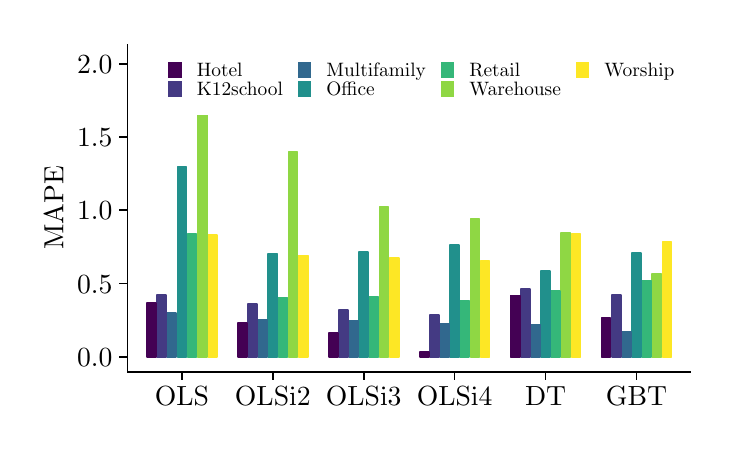
\begin{tikzpicture}[x=1pt,y=1pt]
\definecolor{fillColor}{RGB}{255,255,255}
\path[use as bounding box,fill=fillColor,fill opacity=0.00] (0,0) rectangle (245.72,144.54);
\begin{scope}
\path[clip] (  0.00,  0.00) rectangle (245.72,144.54);
\definecolor{drawColor}{RGB}{255,255,255}
\definecolor{fillColor}{RGB}{255,255,255}

\path[draw=drawColor,line width= 0.6pt,line join=round,line cap=round,fill=fillColor] (  0.00,  0.00) rectangle (245.72,144.54);
\end{scope}
\begin{scope}
\path[clip] ( 36.01, 20.23) rectangle (239.72,138.54);
\definecolor{fillColor}{RGB}{255,255,255}

\path[fill=fillColor] ( 36.01, 20.23) rectangle (239.72,138.54);
\definecolor{drawColor}{RGB}{253,231,37}
\definecolor{fillColor}{RGB}{253,231,37}

\path[draw=drawColor,line width= 0.6pt,line join=round,fill=fillColor] ( 65.06, 25.61) rectangle ( 68.35, 69.67);
\definecolor{drawColor}{RGB}{143,215,68}
\definecolor{fillColor}{RGB}{143,215,68}

\path[draw=drawColor,line width= 0.6pt,line join=round,fill=fillColor] ( 61.40, 25.61) rectangle ( 64.69,133.16);
\definecolor{drawColor}{RGB}{53,183,121}
\definecolor{fillColor}{RGB}{53,183,121}

\path[draw=drawColor,line width= 0.6pt,line join=round,fill=fillColor] ( 57.74, 25.61) rectangle ( 61.02, 69.99);
\definecolor{drawColor}{RGB}{33,144,140}
\definecolor{fillColor}{RGB}{33,144,140}

\path[draw=drawColor,line width= 0.6pt,line join=round,fill=fillColor] ( 54.08, 25.61) rectangle ( 57.36, 94.24);
\definecolor{drawColor}{RGB}{49,104,142}
\definecolor{fillColor}{RGB}{49,104,142}

\path[draw=drawColor,line width= 0.6pt,line join=round,fill=fillColor] ( 50.42, 25.61) rectangle ( 53.70, 41.39);
\definecolor{drawColor}{RGB}{68,58,131}
\definecolor{fillColor}{RGB}{68,58,131}

\path[draw=drawColor,line width= 0.6pt,line join=round,fill=fillColor] ( 46.75, 25.61) rectangle ( 50.04, 47.90);
\definecolor{drawColor}{RGB}{68,1,84}
\definecolor{fillColor}{RGB}{68,1,84}

\path[draw=drawColor,line width= 0.6pt,line join=round,fill=fillColor] ( 43.09, 25.61) rectangle ( 46.38, 45.10);
\definecolor{drawColor}{RGB}{253,231,37}
\definecolor{fillColor}{RGB}{253,231,37}

\path[draw=drawColor,line width= 0.6pt,line join=round,fill=fillColor] ( 97.92, 25.61) rectangle (101.20, 62.20);
\definecolor{drawColor}{RGB}{143,215,68}
\definecolor{fillColor}{RGB}{143,215,68}

\path[draw=drawColor,line width= 0.6pt,line join=round,fill=fillColor] ( 94.26, 25.61) rectangle ( 97.54, 99.54);
\definecolor{drawColor}{RGB}{53,183,121}
\definecolor{fillColor}{RGB}{53,183,121}

\path[draw=drawColor,line width= 0.6pt,line join=round,fill=fillColor] ( 90.60, 25.61) rectangle ( 93.88, 47.00);
\definecolor{drawColor}{RGB}{33,144,140}
\definecolor{fillColor}{RGB}{33,144,140}

\path[draw=drawColor,line width= 0.6pt,line join=round,fill=fillColor] ( 86.93, 25.61) rectangle ( 90.22, 62.84);
\definecolor{drawColor}{RGB}{49,104,142}
\definecolor{fillColor}{RGB}{49,104,142}

\path[draw=drawColor,line width= 0.6pt,line join=round,fill=fillColor] ( 83.27, 25.61) rectangle ( 86.56, 39.06);
\definecolor{drawColor}{RGB}{68,58,131}
\definecolor{fillColor}{RGB}{68,58,131}

\path[draw=drawColor,line width= 0.6pt,line join=round,fill=fillColor] ( 79.61, 25.61) rectangle ( 82.90, 44.73);
\definecolor{drawColor}{RGB}{68,1,84}
\definecolor{fillColor}{RGB}{68,1,84}

\path[draw=drawColor,line width= 0.6pt,line join=round,fill=fillColor] ( 75.95, 25.61) rectangle ( 79.24, 37.84);
\definecolor{drawColor}{RGB}{253,231,37}
\definecolor{fillColor}{RGB}{253,231,37}

\path[draw=drawColor,line width= 0.6pt,line join=round,fill=fillColor] (130.77, 25.61) rectangle (134.06, 61.20);
\definecolor{drawColor}{RGB}{143,215,68}
\definecolor{fillColor}{RGB}{143,215,68}

\path[draw=drawColor,line width= 0.6pt,line join=round,fill=fillColor] (127.11, 25.61) rectangle (130.40, 79.62);
\definecolor{drawColor}{RGB}{53,183,121}
\definecolor{fillColor}{RGB}{53,183,121}

\path[draw=drawColor,line width= 0.6pt,line join=round,fill=fillColor] (123.45, 25.61) rectangle (126.74, 47.16);
\definecolor{drawColor}{RGB}{33,144,140}
\definecolor{fillColor}{RGB}{33,144,140}

\path[draw=drawColor,line width= 0.6pt,line join=round,fill=fillColor] (119.79, 25.61) rectangle (123.08, 63.53);
\definecolor{drawColor}{RGB}{49,104,142}
\definecolor{fillColor}{RGB}{49,104,142}

\path[draw=drawColor,line width= 0.6pt,line join=round,fill=fillColor] (116.13, 25.61) rectangle (119.42, 38.74);
\definecolor{drawColor}{RGB}{68,58,131}
\definecolor{fillColor}{RGB}{68,58,131}

\path[draw=drawColor,line width= 0.6pt,line join=round,fill=fillColor] (112.47, 25.61) rectangle (115.75, 42.61);
\definecolor{drawColor}{RGB}{68,1,84}
\definecolor{fillColor}{RGB}{68,1,84}

\path[draw=drawColor,line width= 0.6pt,line join=round,fill=fillColor] (108.81, 25.61) rectangle (112.09, 34.29);
\definecolor{drawColor}{RGB}{253,231,37}
\definecolor{fillColor}{RGB}{253,231,37}

\path[draw=drawColor,line width= 0.6pt,line join=round,fill=fillColor] (163.63, 25.61) rectangle (166.92, 60.19);
\definecolor{drawColor}{RGB}{143,215,68}
\definecolor{fillColor}{RGB}{143,215,68}

\path[draw=drawColor,line width= 0.6pt,line join=round,fill=fillColor] (159.97, 25.61) rectangle (163.26, 75.39);
\definecolor{drawColor}{RGB}{53,183,121}
\definecolor{fillColor}{RGB}{53,183,121}

\path[draw=drawColor,line width= 0.6pt,line join=round,fill=fillColor] (156.31, 25.61) rectangle (159.59, 45.94);
\definecolor{drawColor}{RGB}{33,144,140}
\definecolor{fillColor}{RGB}{33,144,140}

\path[draw=drawColor,line width= 0.6pt,line join=round,fill=fillColor] (152.65, 25.61) rectangle (155.93, 65.91);
\definecolor{drawColor}{RGB}{49,104,142}
\definecolor{fillColor}{RGB}{49,104,142}

\path[draw=drawColor,line width= 0.6pt,line join=round,fill=fillColor] (148.99, 25.61) rectangle (152.27, 37.68);
\definecolor{drawColor}{RGB}{68,58,131}
\definecolor{fillColor}{RGB}{68,58,131}

\path[draw=drawColor,line width= 0.6pt,line join=round,fill=fillColor] (145.33, 25.61) rectangle (148.61, 40.81);
\definecolor{drawColor}{RGB}{68,1,84}
\definecolor{fillColor}{RGB}{68,1,84}

\path[draw=drawColor,line width= 0.6pt,line join=round,fill=fillColor] (141.66, 25.61) rectangle (144.95, 27.25);
\definecolor{drawColor}{RGB}{253,231,37}
\definecolor{fillColor}{RGB}{253,231,37}

\path[draw=drawColor,line width= 0.6pt,line join=round,fill=fillColor] (196.49, 25.61) rectangle (199.77, 70.04);
\definecolor{drawColor}{RGB}{143,215,68}
\definecolor{fillColor}{RGB}{143,215,68}

\path[draw=drawColor,line width= 0.6pt,line join=round,fill=fillColor] (192.83, 25.61) rectangle (196.11, 70.41);
\definecolor{drawColor}{RGB}{53,183,121}
\definecolor{fillColor}{RGB}{53,183,121}

\path[draw=drawColor,line width= 0.6pt,line join=round,fill=fillColor] (189.17, 25.61) rectangle (192.45, 49.28);
\definecolor{drawColor}{RGB}{33,144,140}
\definecolor{fillColor}{RGB}{33,144,140}

\path[draw=drawColor,line width= 0.6pt,line join=round,fill=fillColor] (185.50, 25.61) rectangle (188.79, 56.64);
\definecolor{drawColor}{RGB}{49,104,142}
\definecolor{fillColor}{RGB}{49,104,142}

\path[draw=drawColor,line width= 0.6pt,line join=round,fill=fillColor] (181.84, 25.61) rectangle (185.13, 37.31);
\definecolor{drawColor}{RGB}{68,58,131}
\definecolor{fillColor}{RGB}{68,58,131}

\path[draw=drawColor,line width= 0.6pt,line join=round,fill=fillColor] (178.18, 25.61) rectangle (181.47, 50.07);
\definecolor{drawColor}{RGB}{68,1,84}
\definecolor{fillColor}{RGB}{68,1,84}

\path[draw=drawColor,line width= 0.6pt,line join=round,fill=fillColor] (174.52, 25.61) rectangle (177.81, 47.80);
\definecolor{drawColor}{RGB}{253,231,37}
\definecolor{fillColor}{RGB}{253,231,37}

\path[draw=drawColor,line width= 0.6pt,line join=round,fill=fillColor] (229.34, 25.61) rectangle (232.63, 67.07);
\definecolor{drawColor}{RGB}{143,215,68}
\definecolor{fillColor}{RGB}{143,215,68}

\path[draw=drawColor,line width= 0.6pt,line join=round,fill=fillColor] (225.68, 25.61) rectangle (228.97, 55.53);
\definecolor{drawColor}{RGB}{53,183,121}
\definecolor{fillColor}{RGB}{53,183,121}

\path[draw=drawColor,line width= 0.6pt,line join=round,fill=fillColor] (222.02, 25.61) rectangle (225.31, 53.20);
\definecolor{drawColor}{RGB}{33,144,140}
\definecolor{fillColor}{RGB}{33,144,140}

\path[draw=drawColor,line width= 0.6pt,line join=round,fill=fillColor] (218.36, 25.61) rectangle (221.65, 63.00);
\definecolor{drawColor}{RGB}{49,104,142}
\definecolor{fillColor}{RGB}{49,104,142}

\path[draw=drawColor,line width= 0.6pt,line join=round,fill=fillColor] (214.70, 25.61) rectangle (217.99, 34.72);
\definecolor{drawColor}{RGB}{68,58,131}
\definecolor{fillColor}{RGB}{68,58,131}

\path[draw=drawColor,line width= 0.6pt,line join=round,fill=fillColor] (211.04, 25.61) rectangle (214.32, 48.01);
\definecolor{drawColor}{RGB}{68,1,84}
\definecolor{fillColor}{RGB}{68,1,84}

\path[draw=drawColor,line width= 0.6pt,line join=round,fill=fillColor] (207.38, 25.61) rectangle (210.66, 39.54);
\end{scope}
\begin{scope}
\path[clip] (  0.00,  0.00) rectangle (245.72,144.54);
\definecolor{drawColor}{RGB}{0,0,0}

\path[draw=drawColor,line width= 0.6pt,line join=round] ( 36.01, 20.23) --
	( 36.01,138.54);
\end{scope}
\begin{scope}
\path[clip] (  0.00,  0.00) rectangle (245.72,144.54);
\definecolor{drawColor}{RGB}{0,0,0}

\node[text=drawColor,anchor=base east,inner sep=0pt, outer sep=0pt, scale=  1.00] at ( 30.61, 22.17) {0.0};

\node[text=drawColor,anchor=base east,inner sep=0pt, outer sep=0pt, scale=  1.00] at ( 30.61, 48.64) {0.5};

\node[text=drawColor,anchor=base east,inner sep=0pt, outer sep=0pt, scale=  1.00] at ( 30.61, 75.12) {1.0};

\node[text=drawColor,anchor=base east,inner sep=0pt, outer sep=0pt, scale=  1.00] at ( 30.61,101.60) {1.5};

\node[text=drawColor,anchor=base east,inner sep=0pt, outer sep=0pt, scale=  1.00] at ( 30.61,128.08) {2.0};
\end{scope}
\begin{scope}
\path[clip] (  0.00,  0.00) rectangle (245.72,144.54);
\definecolor{drawColor}{RGB}{0,0,0}

\path[draw=drawColor,line width= 0.6pt,line join=round] ( 33.01, 25.61) --
	( 36.01, 25.61);

\path[draw=drawColor,line width= 0.6pt,line join=round] ( 33.01, 52.09) --
	( 36.01, 52.09);

\path[draw=drawColor,line width= 0.6pt,line join=round] ( 33.01, 78.56) --
	( 36.01, 78.56);

\path[draw=drawColor,line width= 0.6pt,line join=round] ( 33.01,105.04) --
	( 36.01,105.04);

\path[draw=drawColor,line width= 0.6pt,line join=round] ( 33.01,131.52) --
	( 36.01,131.52);
\end{scope}
\begin{scope}
\path[clip] (  0.00,  0.00) rectangle (245.72,144.54);
\definecolor{drawColor}{RGB}{0,0,0}

\path[draw=drawColor,line width= 0.6pt,line join=round] ( 36.01, 20.23) --
	(239.72, 20.23);
\end{scope}
\begin{scope}
\path[clip] (  0.00,  0.00) rectangle (245.72,144.54);
\definecolor{drawColor}{RGB}{0,0,0}

\path[draw=drawColor,line width= 0.6pt,line join=round] ( 55.72, 17.23) --
	( 55.72, 20.23);

\path[draw=drawColor,line width= 0.6pt,line join=round] ( 88.58, 17.23) --
	( 88.58, 20.23);

\path[draw=drawColor,line width= 0.6pt,line join=round] (121.43, 17.23) --
	(121.43, 20.23);

\path[draw=drawColor,line width= 0.6pt,line join=round] (154.29, 17.23) --
	(154.29, 20.23);

\path[draw=drawColor,line width= 0.6pt,line join=round] (187.15, 17.23) --
	(187.15, 20.23);

\path[draw=drawColor,line width= 0.6pt,line join=round] (220.00, 17.23) --
	(220.00, 20.23);
\end{scope}
\begin{scope}
\path[clip] (  0.00,  0.00) rectangle (245.72,144.54);
\definecolor{drawColor}{RGB}{0,0,0}

\node[text=drawColor,anchor=base,inner sep=0pt, outer sep=0pt, scale=  1.00] at ( 55.72,  7.94) {OLS};

\node[text=drawColor,anchor=base,inner sep=0pt, outer sep=0pt, scale=  1.00] at ( 88.58,  7.94) {OLSi2};

\node[text=drawColor,anchor=base,inner sep=0pt, outer sep=0pt, scale=  1.00] at (121.43,  7.94) {OLSi3};

\node[text=drawColor,anchor=base,inner sep=0pt, outer sep=0pt, scale=  1.00] at (154.29,  7.94) {OLSi4};

\node[text=drawColor,anchor=base,inner sep=0pt, outer sep=0pt, scale=  1.00] at (187.15,  7.94) {DT};

\node[text=drawColor,anchor=base,inner sep=0pt, outer sep=0pt, scale=  1.00] at (220.00,  7.94) {GBT};
\end{scope}
\begin{scope}
\path[clip] (  0.00,  0.00) rectangle (245.72,144.54);
\definecolor{drawColor}{RGB}{0,0,0}

\node[text=drawColor,rotate= 90.00,anchor=base west,inner sep=0pt, outer sep=0pt, scale=  1.00] at ( 12.89, 64.25) {MAPE};
\end{scope}
\begin{scope}
\path[clip] (  0.00,  0.00) rectangle (245.72,144.54);
\definecolor{fillColor}{RGB}{255,255,255}

\path[fill=fillColor] ( 39.41,113.01) rectangle (239.72,138.54);
\end{scope}
\begin{scope}
\path[clip] (  0.00,  0.00) rectangle (245.72,144.54);
\definecolor{drawColor}{RGB}{68,1,84}
\definecolor{fillColor}{RGB}{68,1,84}

\path[draw=drawColor,line width= 0.6pt,line cap=round,fill=fillColor] ( 51.13,126.49) rectangle ( 55.39,131.83);
\end{scope}
\begin{scope}
\path[clip] (  0.00,  0.00) rectangle (245.72,144.54);
\definecolor{drawColor}{RGB}{68,58,131}
\definecolor{fillColor}{RGB}{68,58,131}

\path[draw=drawColor,line width= 0.6pt,line cap=round,fill=fillColor] ( 51.13,119.72) rectangle ( 55.39,125.06);
\end{scope}
\begin{scope}
\path[clip] (  0.00,  0.00) rectangle (245.72,144.54);
\definecolor{drawColor}{RGB}{49,104,142}
\definecolor{fillColor}{RGB}{49,104,142}

\path[draw=drawColor,line width= 0.6pt,line cap=round,fill=fillColor] ( 97.96,126.49) rectangle (102.23,131.83);
\end{scope}
\begin{scope}
\path[clip] (  0.00,  0.00) rectangle (245.72,144.54);
\definecolor{drawColor}{RGB}{33,144,140}
\definecolor{fillColor}{RGB}{33,144,140}

\path[draw=drawColor,line width= 0.6pt,line cap=round,fill=fillColor] ( 97.96,119.72) rectangle (102.23,125.06);
\end{scope}
\begin{scope}
\path[clip] (  0.00,  0.00) rectangle (245.72,144.54);
\definecolor{drawColor}{RGB}{53,183,121}
\definecolor{fillColor}{RGB}{53,183,121}

\path[draw=drawColor,line width= 0.6pt,line cap=round,fill=fillColor] (149.61,126.49) rectangle (153.88,131.83);
\end{scope}
\begin{scope}
\path[clip] (  0.00,  0.00) rectangle (245.72,144.54);
\definecolor{drawColor}{RGB}{143,215,68}
\definecolor{fillColor}{RGB}{143,215,68}

\path[draw=drawColor,line width= 0.6pt,line cap=round,fill=fillColor] (149.61,119.72) rectangle (153.88,125.06);
\end{scope}
\begin{scope}
\path[clip] (  0.00,  0.00) rectangle (245.72,144.54);
\definecolor{drawColor}{RGB}{253,231,37}
\definecolor{fillColor}{RGB}{253,231,37}

\path[draw=drawColor,line width= 0.6pt,line cap=round,fill=fillColor] (198.41,126.49) rectangle (202.68,131.83);
\end{scope}
\begin{scope}
\path[clip] (  0.00,  0.00) rectangle (245.72,144.54);
\definecolor{drawColor}{RGB}{0,0,0}

\node[text=drawColor,anchor=base west,inner sep=0pt, outer sep=0pt, scale=  0.70] at ( 61.11,126.75) {Hotel};
\end{scope}
\begin{scope}
\path[clip] (  0.00,  0.00) rectangle (245.72,144.54);
\definecolor{drawColor}{RGB}{0,0,0}

\node[text=drawColor,anchor=base west,inner sep=0pt, outer sep=0pt, scale=  0.70] at ( 61.11,119.98) {K12school};
\end{scope}
\begin{scope}
\path[clip] (  0.00,  0.00) rectangle (245.72,144.54);
\definecolor{drawColor}{RGB}{0,0,0}

\node[text=drawColor,anchor=base west,inner sep=0pt, outer sep=0pt, scale=  0.70] at (107.94,126.75) {Multifamily};
\end{scope}
\begin{scope}
\path[clip] (  0.00,  0.00) rectangle (245.72,144.54);
\definecolor{drawColor}{RGB}{0,0,0}

\node[text=drawColor,anchor=base west,inner sep=0pt, outer sep=0pt, scale=  0.70] at (107.94,119.98) {Office};
\end{scope}
\begin{scope}
\path[clip] (  0.00,  0.00) rectangle (245.72,144.54);
\definecolor{drawColor}{RGB}{0,0,0}

\node[text=drawColor,anchor=base west,inner sep=0pt, outer sep=0pt, scale=  0.70] at (159.59,126.75) {Retail};
\end{scope}
\begin{scope}
\path[clip] (  0.00,  0.00) rectangle (245.72,144.54);
\definecolor{drawColor}{RGB}{0,0,0}

\node[text=drawColor,anchor=base west,inner sep=0pt, outer sep=0pt, scale=  0.70] at (159.59,119.98) {Warehouse};
\end{scope}
\begin{scope}
\path[clip] (  0.00,  0.00) rectangle (245.72,144.54);
\definecolor{drawColor}{RGB}{0,0,0}

\node[text=drawColor,anchor=base west,inner sep=0pt, outer sep=0pt, scale=  0.70] at (208.39,126.75) {Worship};
\end{scope}
\end{tikzpicture}
